\documentclass[catalan, a4paper, nobib]{tufte-handout}

% encoding
\usepackage[utf8]{inputenc}
\usepackage[T1]{fontenc}
\usepackage{lmodern}
\usepackage{babel}
\usepackage{pdfpages}
\usepackage{xfrac}

\frenchspacing
\usepackage[style=spanish]{csquotes}
\MakeAutoQuote{«}{»}

\usepackage{booktabs}
\usepackage{circuitikz}
\usepackage{siunitx}
\usepackage{amsmath}

\graphicspath{
    {fotos/}
}

% hyperlink setup / metadata
\usepackage{hyperref}
\AfterPreamble{\hypersetup{
  %%pdfauthor={},
  %%pdftitle={},
  %%pdfsubject={},
}}

% document metadata
\author{Sofija Starcevic i Víctor Méndez}
\title{FISE: Pràctica 5}
\date{22-4-2024}

\begin{document}

\maketitle

\part{Primera sessió}
\newthought{Qüestió L4.1: } A la simulació s'observa $f_o\simeq\qty{1}{\kilo\hertz}$, $BW\simeq\qty{3}{\kilo\hertz}$, $Q=\sfrac{1}{3}$ i un guany $G=\sfrac{1}{3}$.

\begin{figure}[!h]
    \begin{center}
        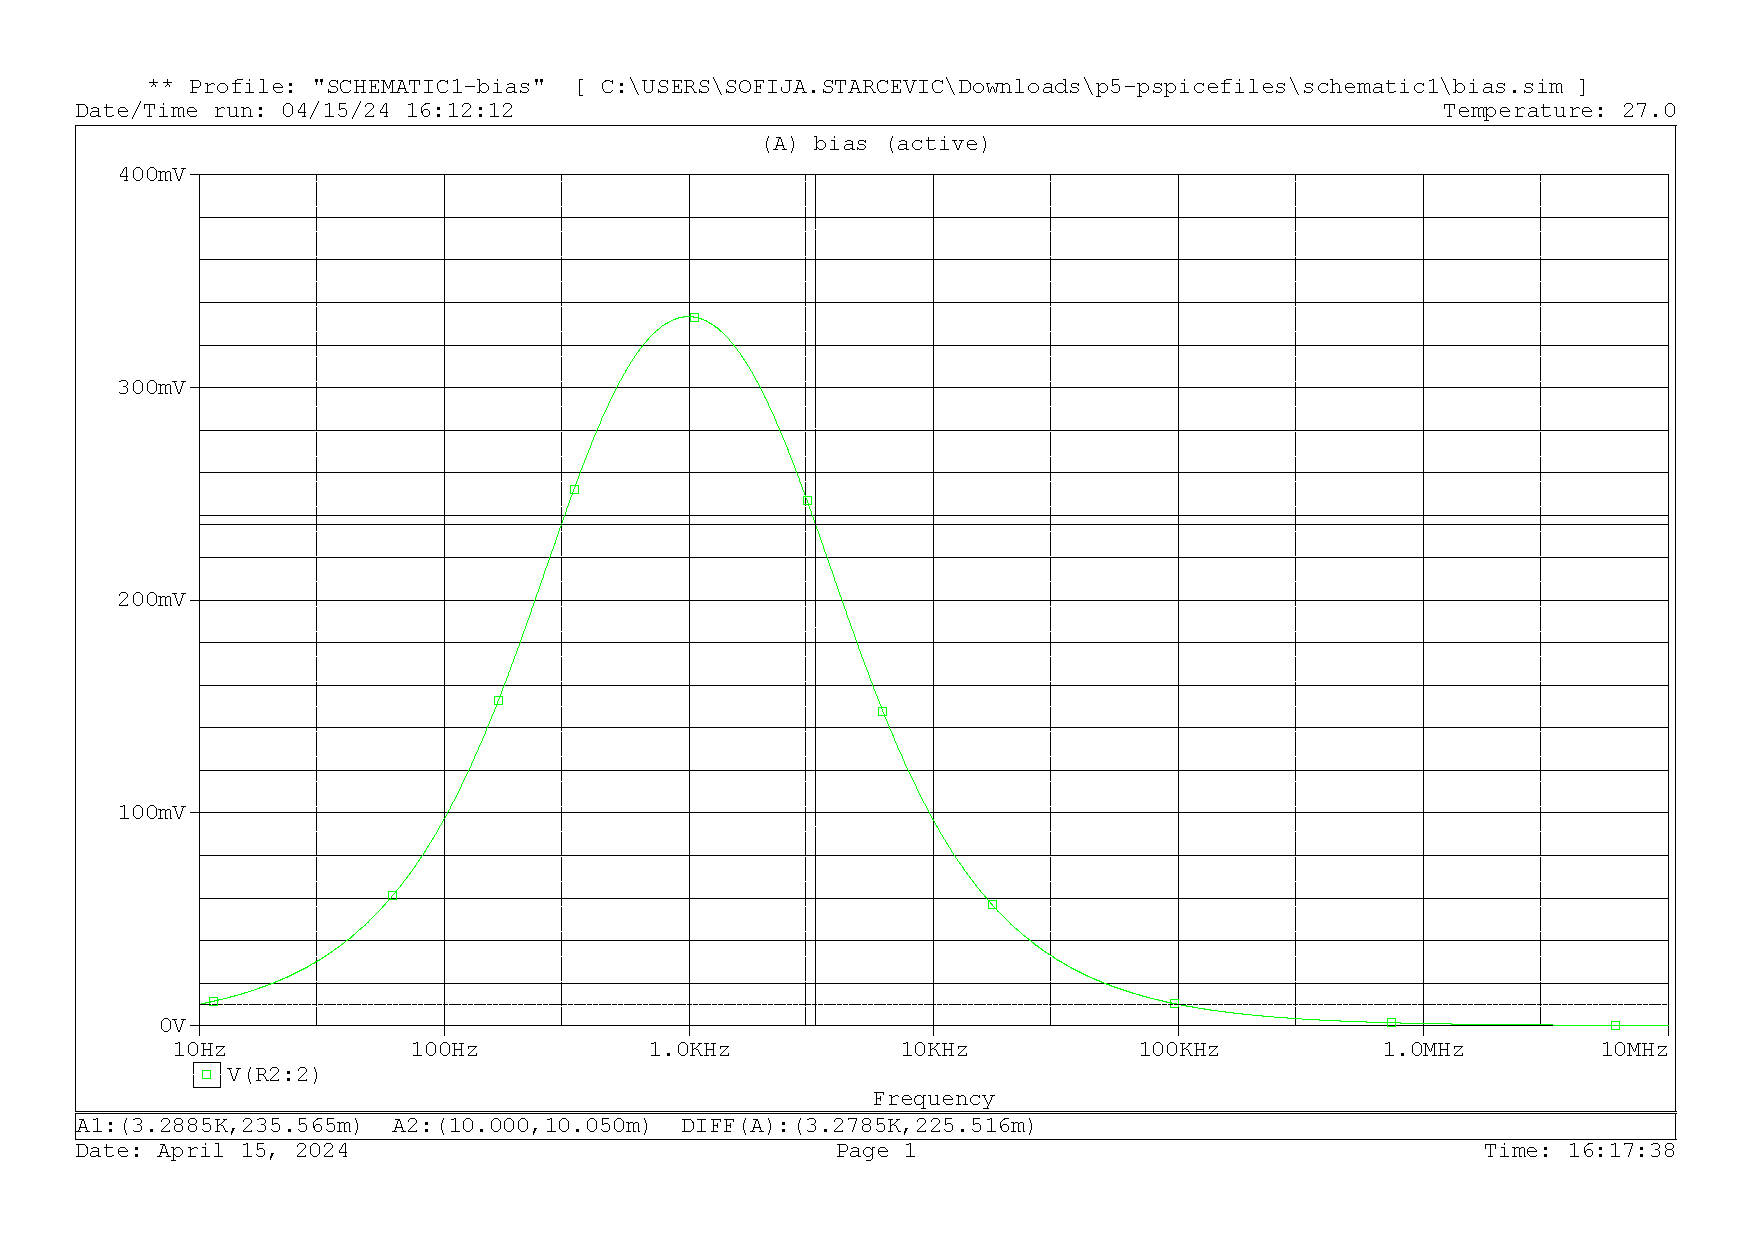
\includegraphics[width=275px]{1.pdf}
    \end{center}
    \caption{Resposta freqüencial del filtre passiu}
\end{figure}

\newthought{Qüestió L4.2: } El factor de qualitat simulat val $Q\simeq\num{5.26}$ tal com es volia i com s'ha calculat a l'estudi previ. Les freqüències de tall son $f_c^-=\qty{900}{\hertz}$ i $f_c^+=\qty{1.09}{\kilo\hertz}$. L'amplada val $BW=f_c^+-f_c^-=\qty{190}{\hertz}$ i el guany $G=\qty{20}{\deci\bel}$. Molt més selectiu que el filtre passiu.

\begin{figure}
    \begin{center}
        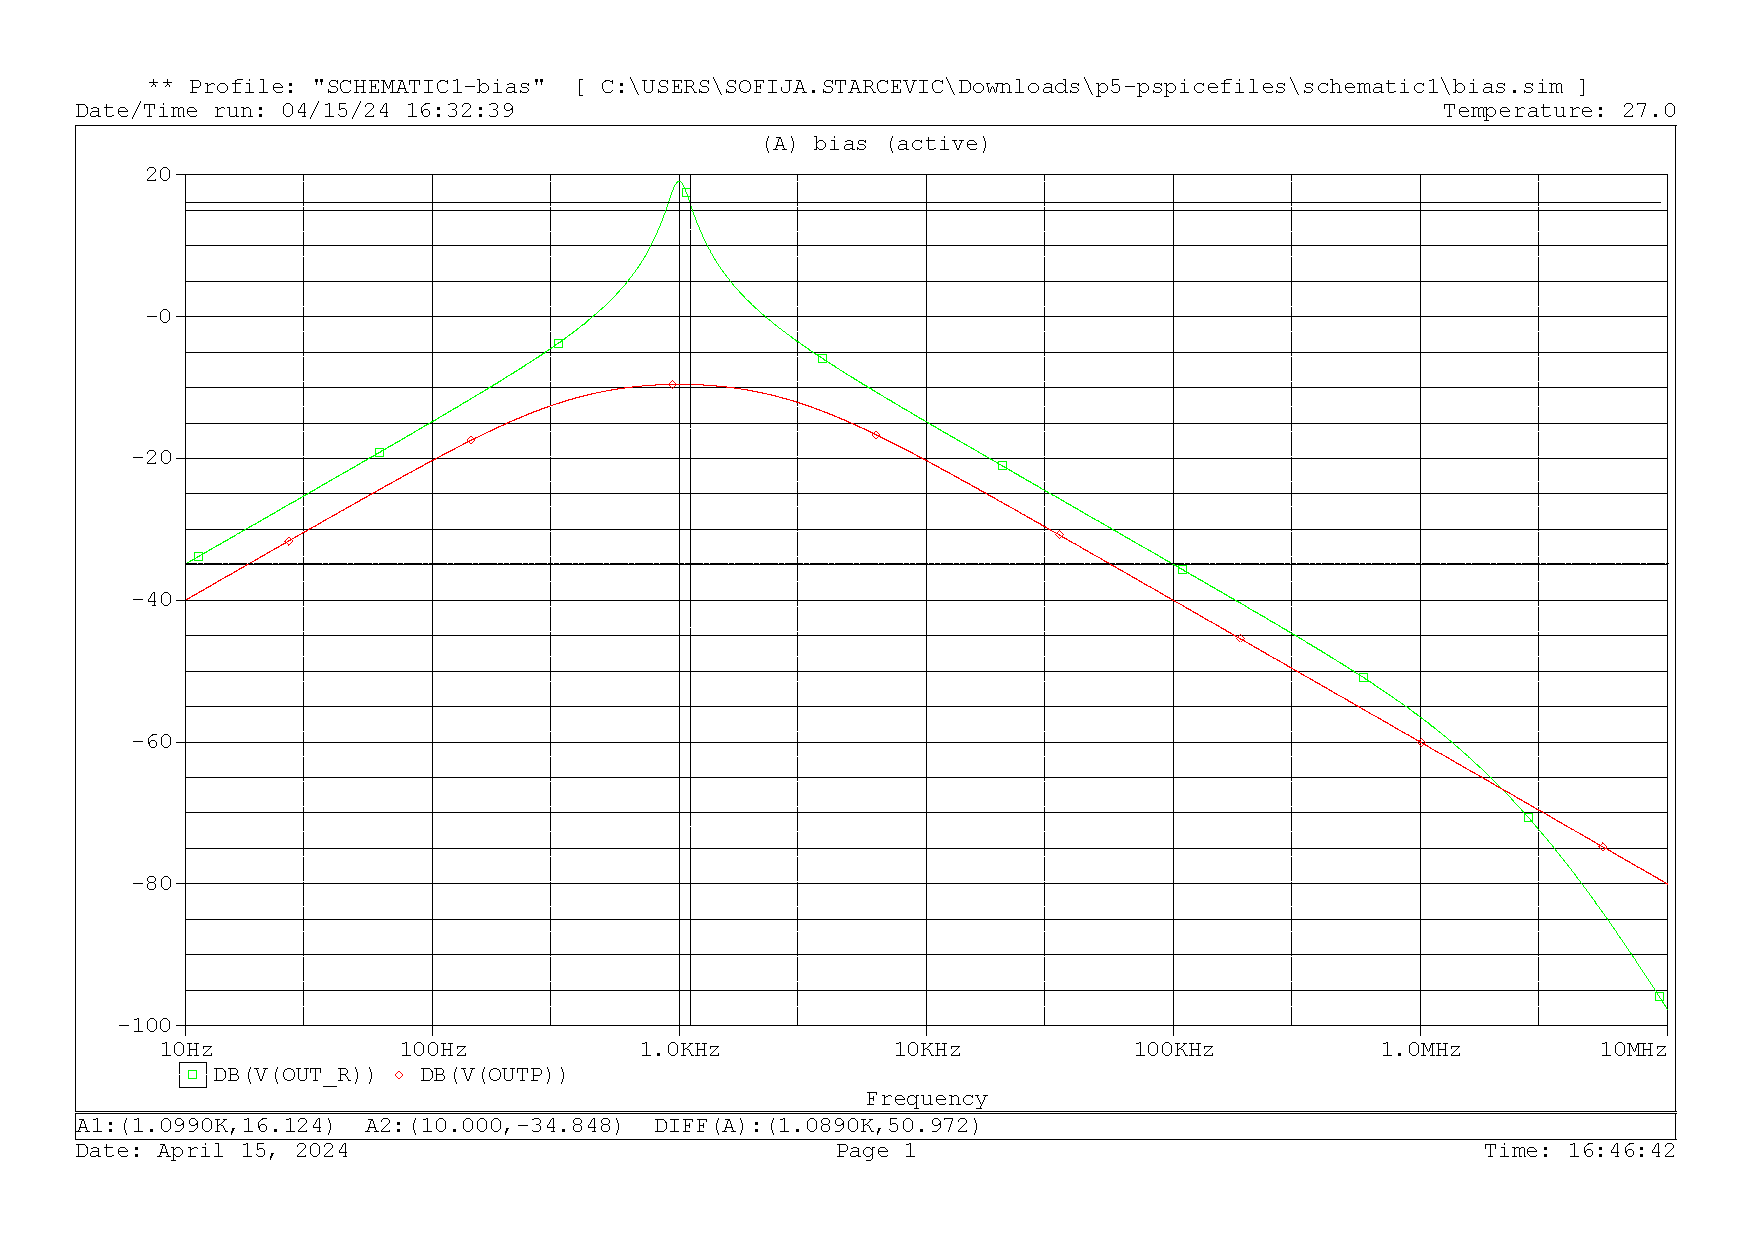
\includegraphics[width=275px]{2.pdf}
    \end{center}
    \caption{Superposició de la resposta freqüencial del filtre passiu i el filtre realimentat}
\end{figure}

\newpage

\newthought{Qüestió L4.3: } Veure la figura \ref{fig:variable_c} i la taula \ref{tab:variable_c}.

\begin{table}[!h]
    \begin{center}
      \begin{tabular}{@{}rccc@{}}
        \toprule
        $C_i$ & \qty{0.1}{\nano\farad} & \qty{1}{\nano\farad} & \qty{10}{\nano\farad} \\
        \midrule
        $f_i$ & \qty{90.5}{\kilo\hertz} & \qty{10}{\kilo\hertz} & \qty{1}{\kilo\hertz} \\
        \bottomrule
      \end{tabular}
    \end{center}
    \caption{Freqüència central segons valor de $C$}
    \label{tab:variable_c}
\end{table}

\begin{figure*}[!h]
    \begin{center}
        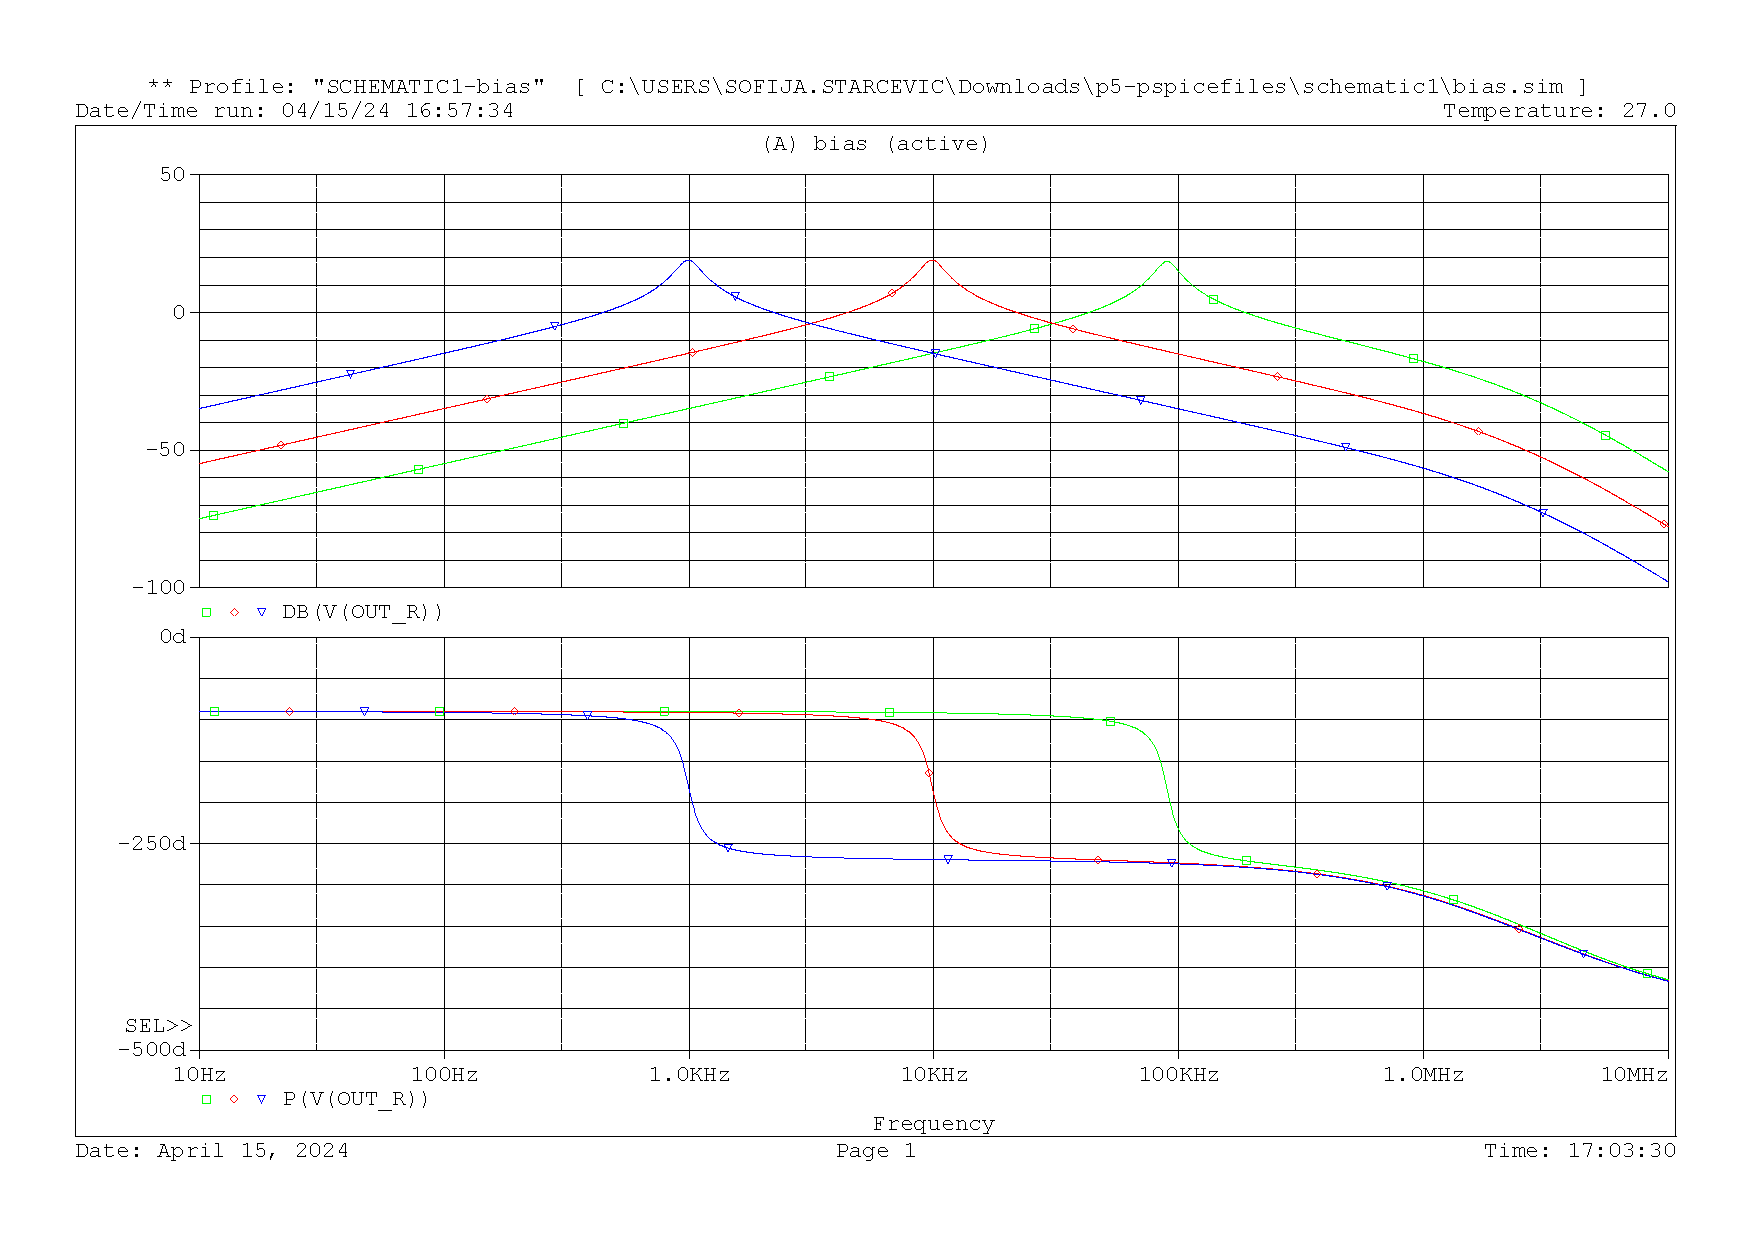
\includegraphics[width=465px]{3.pdf}
    \end{center}
    \caption{Resposta del filtre realimentat per diferents valors de $C$}
    \label{fig:variable_c}
\end{figure*}

\newthought{Qüestió L4.4: } El filtre centrat a \qty{100}{\kilo\hertz} no es pot fer servir. Realment està centrat a \qty{90.5}{\kilo\hertz}. A freqüències altes els pols i ceros del propi AO deixen de ser negligibles i provoquen aquesta diferència entre el càlcul teòric i la simulació.

\newpage

\newthought{Qüestió L5.1: } El circuit s'està començant a comportar com un osci\l.lador en comptes d'un filtre.

\begin{figure}[!h]
    \begin{center}
        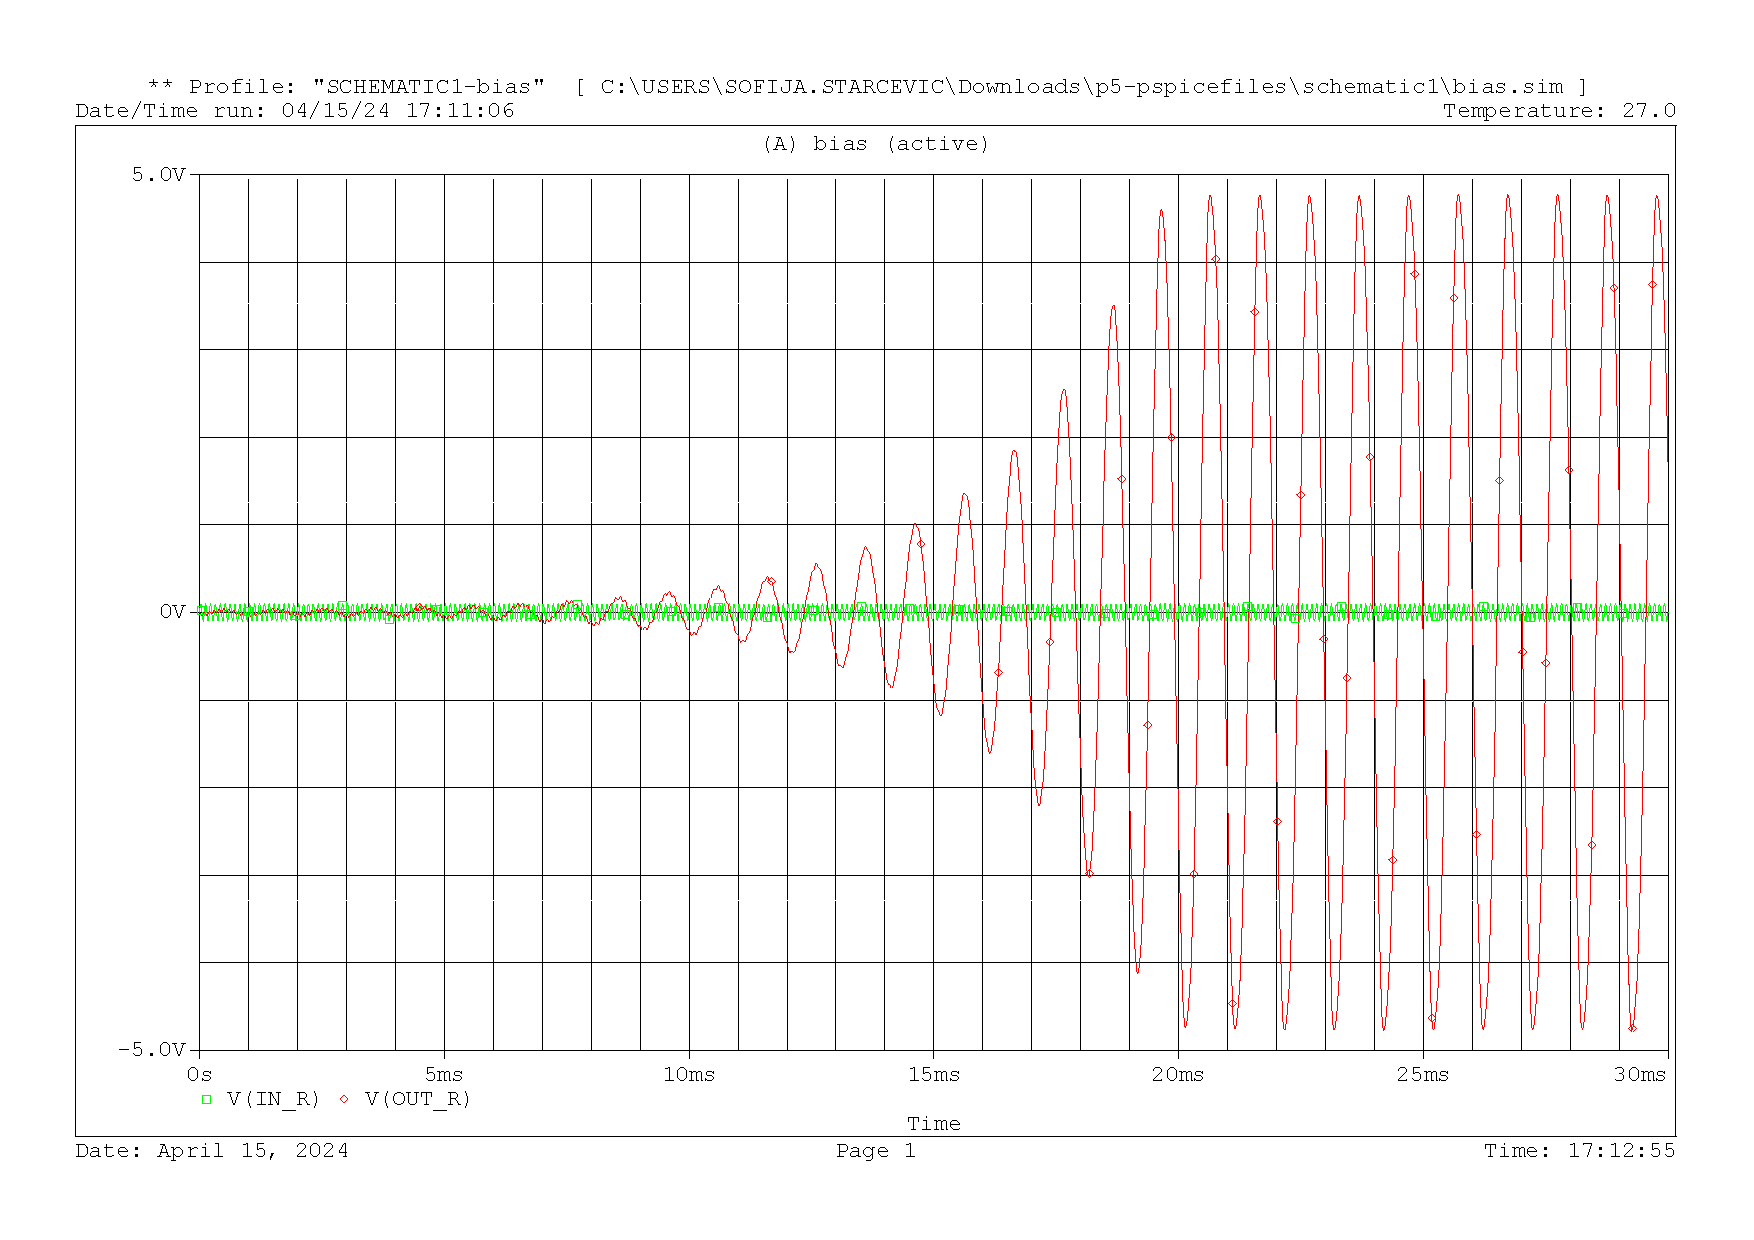
\includegraphics[width=300px]{5.1.pdf}
    \end{center}
    \caption{Filtre en estat d'osci\l.lació}
\end{figure}

\newthought{Qüestió L5.2: } S'obté una freqüència d'osci\l.lació de \qty{1}{\kilo\hertz}.

\begin{figure}[!h]
    \begin{center}
        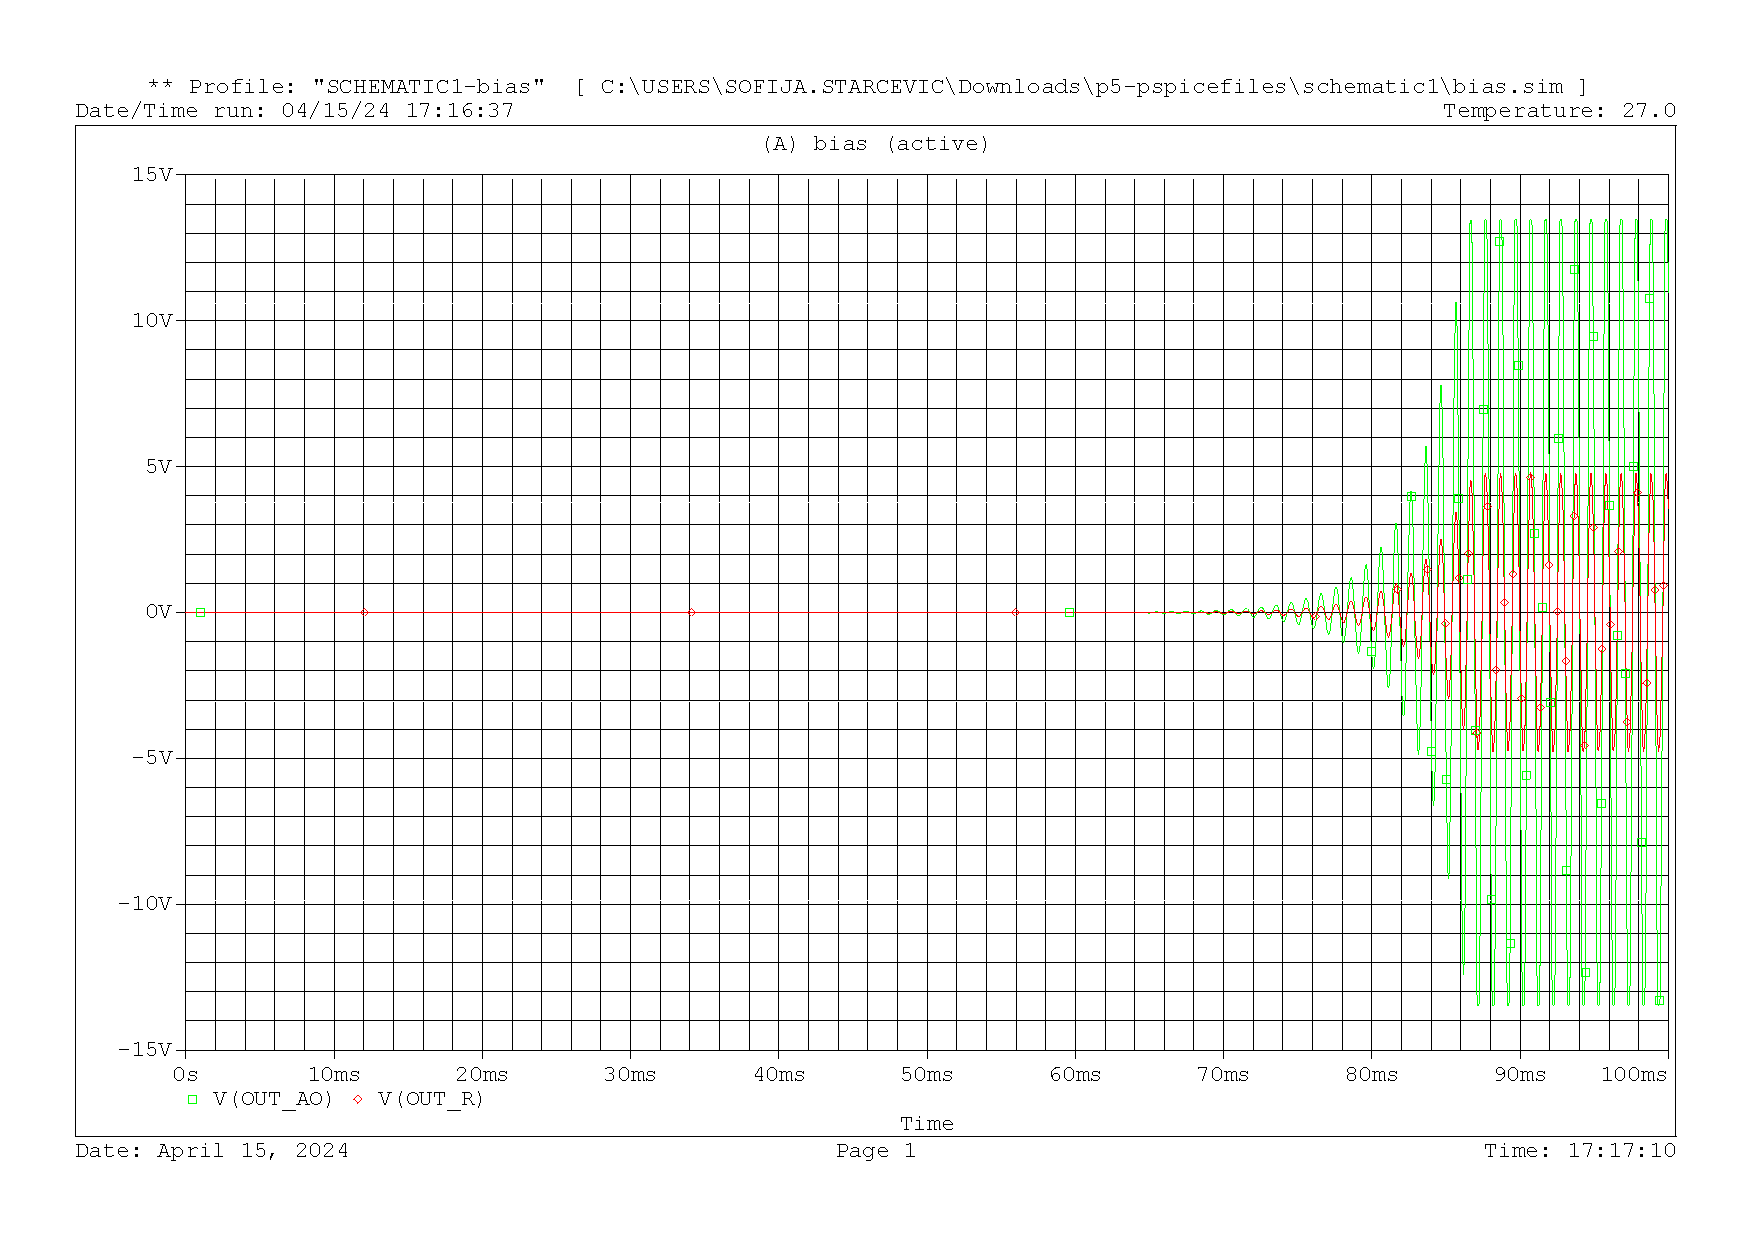
\includegraphics[width=300px]{5.2.pdf}
    \end{center}
    \caption{Osci\l.lació lliure a la sortida del AO i del filtre passiu}
\end{figure}

\newpage

\newthought{Qüestió L5.3: } La freqüència fonamental $f_0 = \qty{1}{\kilo\hertz}$. La relació $R_{0\rightarrow2}=\frac{v_{AO}(f_0)}{v_{AO}(f_2)} = \num{35.75}$.

\begin{figure*}[!h]
    \begin{center}
        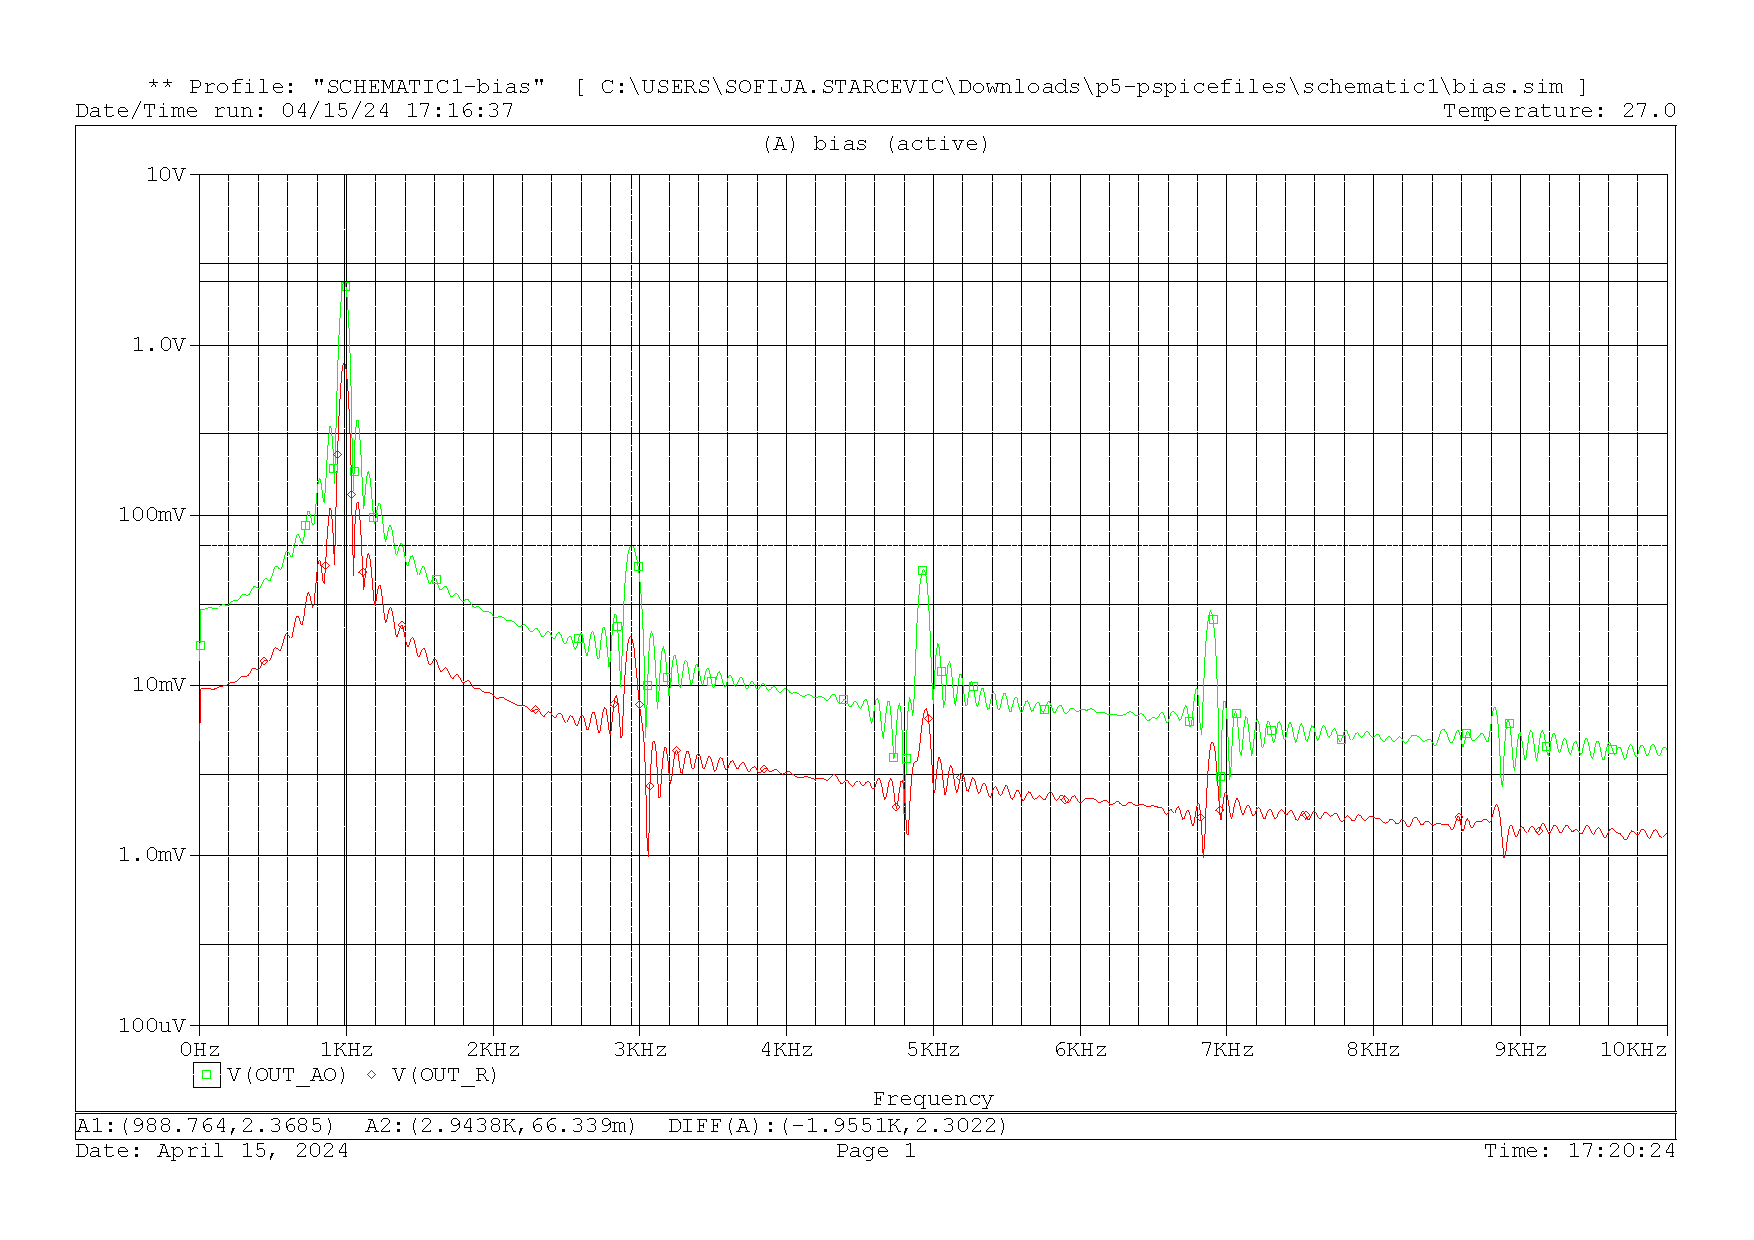
\includegraphics[width=450px]{5.3.pdf}
    \end{center}
    \caption{FFT de l'osci\l.lador}
\end{figure*}

\newthought{Qüestió L5.4: } Quan els dos díodes estan en tall $f_{R1} = \frac{R_F}{R_A}=\num{2.2}$, quen un condueix $f_{R2} = \frac{(R_F//R_B)}{R_A}$. La relació $f_{R2}$ és més petita que $f_{R1}$, i no osci\l.la per aquesta amplificació.

\newthought{Qüestió L5.5: } Veure la taula \ref{tab:variable_r} i figura \ref{fig:variable_r}.

\begin{table}[!h]
    \begin{center}
      \begin{tabular}{@{}rccc@{}}
        \toprule
        $R_i$ & \qty{25}{\kilo\ohm} & \qty{50}{\kilo\ohm} & \qty{100}{\kilo\ohm} \\
        \midrule
        $A_i$ & \qty{190}{\milli\volt} & \qty{225}{\milli\volt} & \qty{350}{\milli\volt} \\
        \bottomrule
      \end{tabular}
    \end{center}
    \caption{Amplitud d'osci\l.lació segons $R$}
    \label{tab:variable_r}
\end{table}

\newpage

\begin{figure*}[!h]
    \begin{center}
        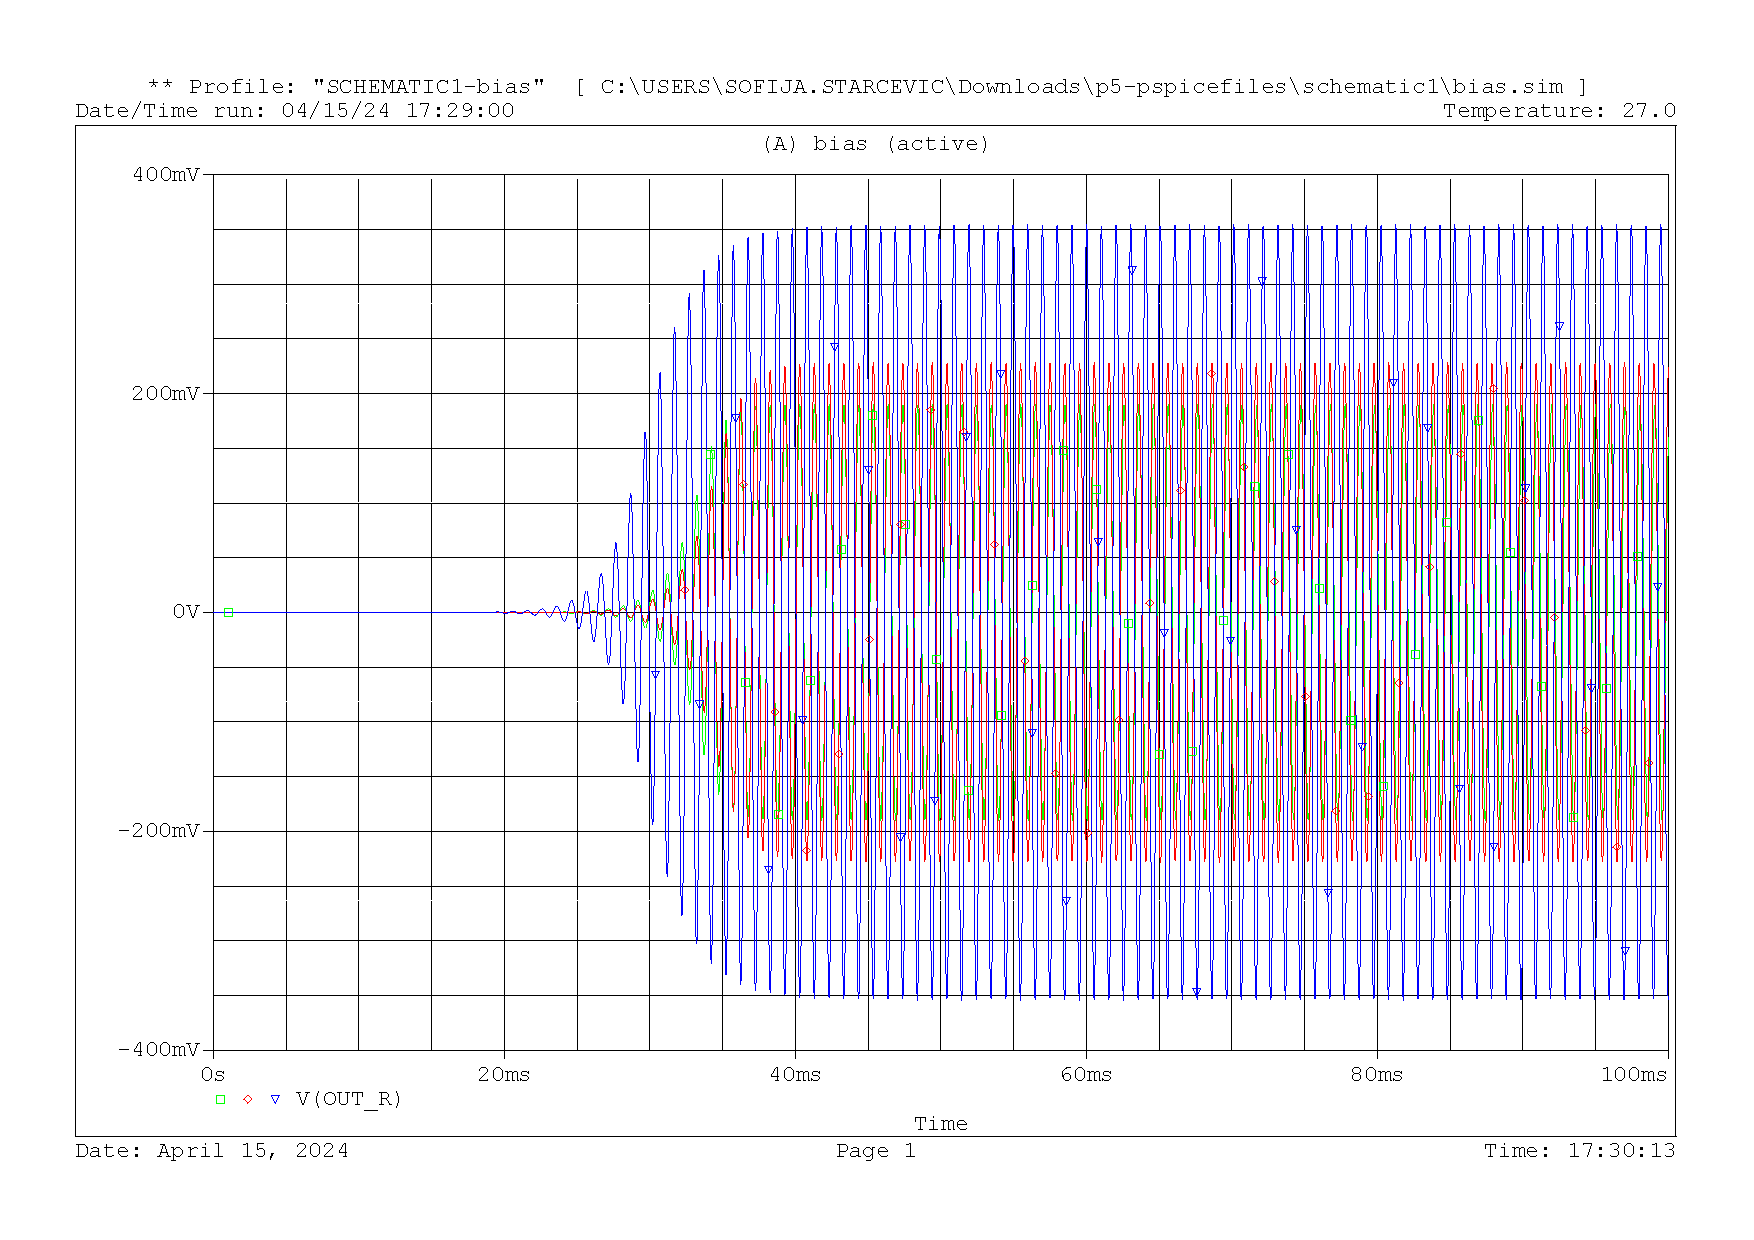
\includegraphics[width=395px]{5.5.pdf}
    \end{center}
    \caption{Osci\l.lació per diferents valors $R$}
    \label{fig:variable_r}
\end{figure*}

\newthought{Qüestió L5.6: } La relació val $R_{0\rightarrow2}=\num{110}$.

\newthought{Qüestió L5.7: } La relació és molt més gran que abans. La distorsió a millorat.

\begin{figure*}[!h]
    \begin{center}
        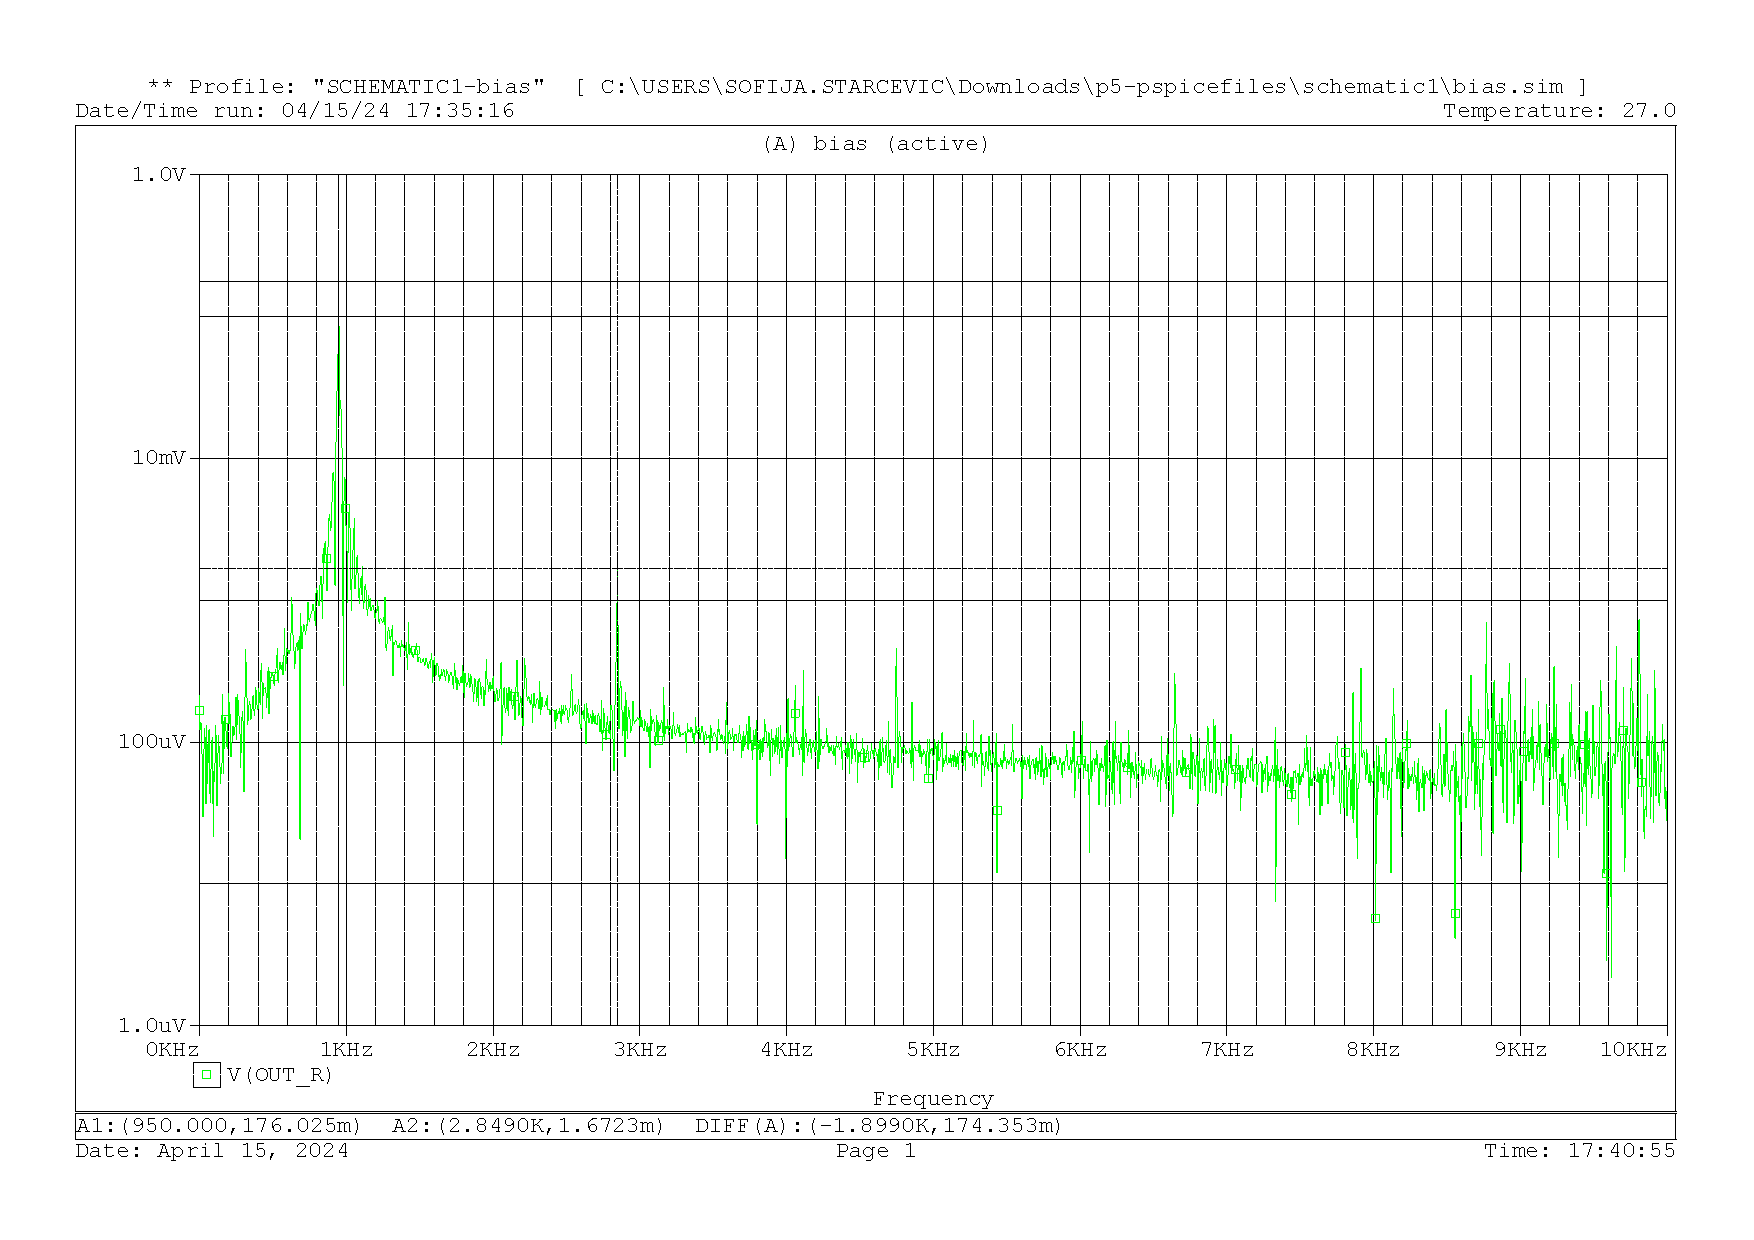
\includegraphics[width=395px]{5.6.pdf}
    \end{center}
    \caption{FFT de osci\l.lador amb estabilització}
\end{figure*}

\newpage

\part{Segona sessió}
\newthought{Qüestió L6.1: } Veure taula \ref{tab:bode} i figura \ref{fig:bode}.

\begin{table}[!h]
    \begin{center}
      \begin{tabular}{@{}rccccc@{}}
        \toprule
        Freqüència & \qty{100}{\hertz} & \qty{200}{\hertz} & \qty{500}{\hertz} & \qty{750}{\hertz} & \qty{900}{\hertz} \\
        \midrule
        Guany$_{\unit{\deci\bel}}$ & \qty{-30.28}{\deci\bel} & \qty{-17.35}{\deci\bel} & \qty{4.93}{\deci\bel} & \qty{22.94}{\deci\bel} & \qty{39.2}{\deci\bel} \\
        \bottomrule
        \toprule
        \qty{1}{\kilo\hertz} & \qty{1.2}{\kilo\hertz} & \qty{1.5}{\kilo\hertz} & \qty{2}{\kilo\hertz} & \qty{5}{\kilo\hertz} & \qty{10}{\kilo\hertz} \\
        \midrule
        \qty{44.49}{\deci\bel} & \qty{28.93}{\deci\bel} & \qty{14.83}{\deci\bel} & \qty{3.81}{\deci\bel} & \qty{-17.35}{\deci\bel} & \qty{-30.74}{\deci\bel} \\
        \bottomrule
      \end{tabular}
    \end{center}
    \caption{Guany en \unit{\deci\bel} segons freqüència}
    \label{tab:bode}
\end{table}

\begin{figure*}[!h]
    \begin{center}
        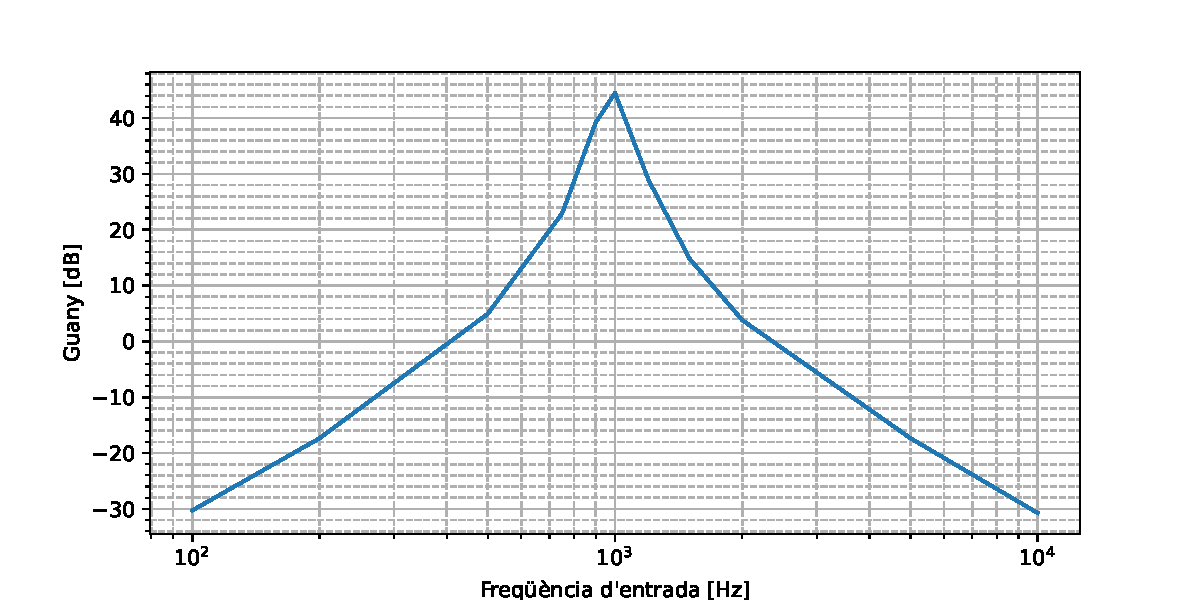
\includegraphics[width=450px]{s2_graph.pdf}
    \end{center}
    \caption{Diagrama de Bode experimental del filtre actiu}
    \label{fig:bode}
\end{figure*}

\newthought{Qüestió L6.2: } La freqüència central val \qty{1}{\kilo\hertz}. El guany val $G_{\unit{\deci\bel}}=\qty{44.49}{\deci\bel}$. A partir de les mesures $f_c^-\simeq\qty{940}{\hertz}$ i $f_c^+\simeq\qty{1.1}{\kilo\hertz}$, per tant $Q = \frac{f_0}{f_c^+-f_c^-}=6.25$.

\newthought{Qüestió L7.1: } Té una freqüència de \qty{4}{\kilo\hertz} i una amplitud de \qty{180}{\milli\volt}. Veure la figura \ref{fig:estable}.

\newthought{Qüestió L7.2: } La resistència del potenciòmetre val \qty{20}{\kilo\hertz}.

\newthought{Qüestió L7.3: } La tensió de sortida osci\l.la a \qty{1}{\kilo\hertz} amb una amplitud de \qty{4.8}{\volt}. Es pot veure un arrisament a la sortida, aquest efecte ve per part de l'entrada. Veure la figura \ref{fig:metaestable}.

\newthought{Qüestió L7.4: } L'arrisament que es veia abans ja no hi és. La sortida és més pura. Veure la figura \ref{fig:metaestable_pur}.

\newthought{Qüestió L7.5: } La sortida és de \qty{1}{\kilo\hertz}, pero té una amplitud de \qty{800}{\milli\volt}. Veure la figura \ref{fig:metaestable_limitat}

\newpage

\begin{figure*}[!h]
    \begin{center}
        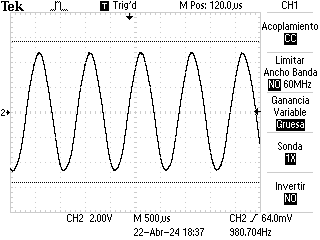
\includegraphics[width=400px]{L7_1.png}
    \end{center}
    \caption{Sortida estable amb el potenciòmetre a mitja cursa}
    \label{fig:estable}
\end{figure*}

\begin{figure*}[!h]
    \begin{center}
        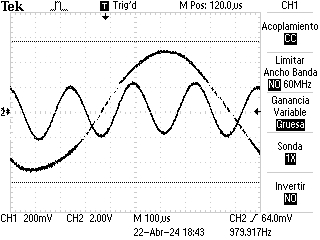
\includegraphics[width=400px]{L7_2.png}
    \end{center}
    \caption{Sortida osci\l.lant amb el potenciòmetre a \qty{20}{\kilo\hertz}}
    \label{fig:metaestable}
\end{figure*}

\newpage

\begin{figure*}[!h]
    \begin{center}
        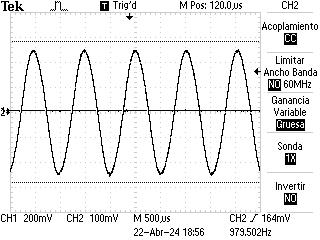
\includegraphics[width=400px]{L7_3.png}
    \end{center}
    \caption{Sortida osci\l.lant pura, amb l'entrada a terra}
    \label{fig:metaestable_pur}
\end{figure*}

\begin{figure*}[!h]
    \begin{center}
        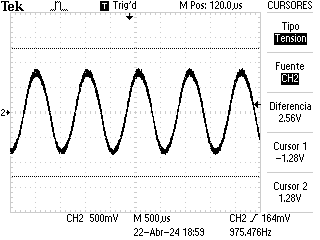
\includegraphics[width=400px]{L8.png}
    \end{center}
    \caption{Sortida osci\l.lant pura amb l'amplitud limitada}
    \label{fig:metaestable_limitat}
\end{figure*}

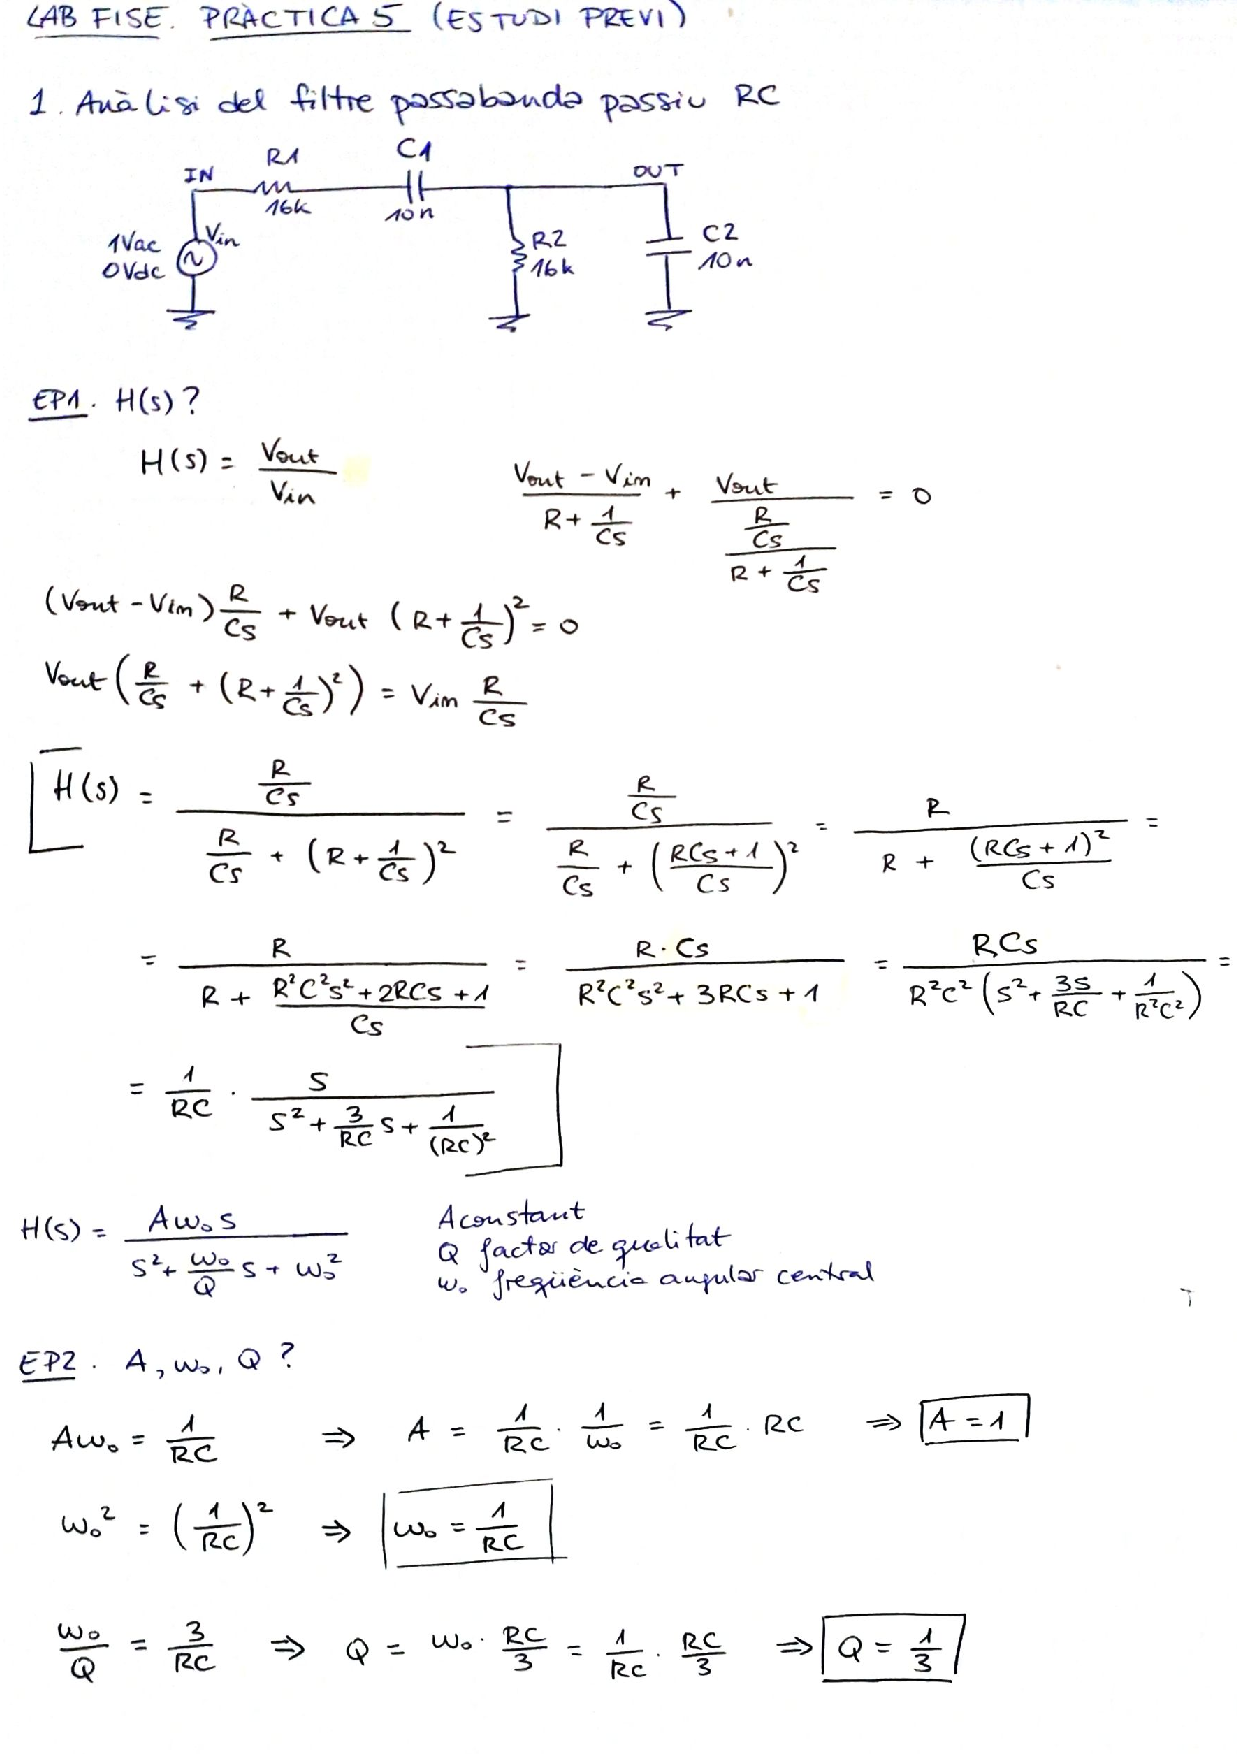
\includepdf[pages={1-6}]{EP_FISE_P5.pdf}

\end{document}